\chapter{Metodologi}

Pada bab ini penulis menjelaskan mengenai metodologi yang digunakan selama pengerjaan tugas akhir.

\begin{figure}[H]
	\begin{centering}
		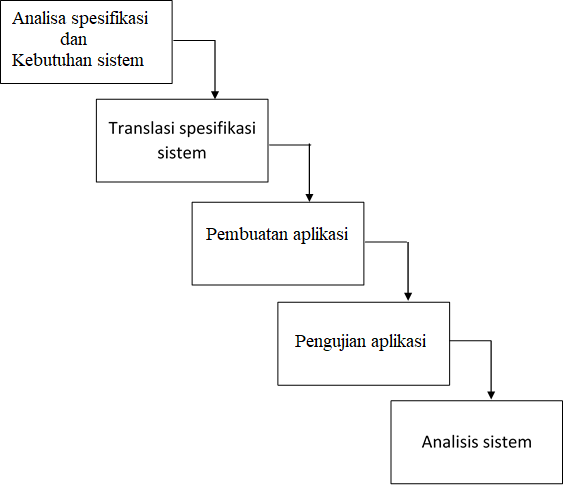
\includegraphics[scale=0.7]{metodologi_proposal}
		
		\caption{Metodologi.}
	\end{centering}
\end{figure}

\section{Analisa spesifikasi dan Kebutuhan sistem}

Menganalisa spesifikasi-spesifikasi pada teka-teki sudoku, lalu membuat kebutuhan dari aplikasi sistem yang akan mengeluarkan \textit{use case} aplikasi.

\section{Translasi spesifikasi sistem}

Spesifikasi yang sudah di dapat diubah dalam bentuk logika proposisi lalu dijadikan dalam bentuk CNF.

\section{Pembuatan aplikasi}

Spesifikasi yang sudah dalam bentuk CNF akan digunakan pada \textit{SAT Solver}. Lalu \textit{use case} yang didapat akan dibuat fungsionalitasnya. Pembuatan aplikasi menggunakan \textit{waterfall design} tahapan-nya berupa:

\subsection{Spesifikasi Aplikasi}

Spesifikai aplikasi adalah sebagai berikut:
\begin{enumerate}
	\item Bermain sudoku.
	\item Membuat sudoku.
	\item Memecahkan sudoku.
\end{enumerate}

\begin{figure}[H]
	\begin{centering}
		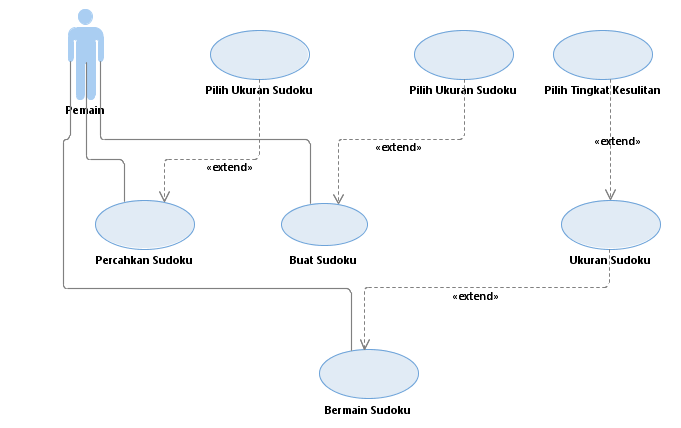
\includegraphics[scale=1]{gambar/useCase}
		
		\caption{\textit{Use Case Diagram}.}
	\end{centering}
\end{figure}

\subsection{\textit{Analysis}}

Dalam \textit{analysis}, penulis menjabarkan mulai dari hal
mendasar yaitu kendala global dalam pengembangan perangkat lunak yang sudah ada. Adapun masalahnya adalah minimnya aplikasi pemecah sudoku yang interaktif.

\subsection{\textit{Design}}

Fitur yang akan ada pada aplikasi tersebut adalah sebagai berikut

 \begin{enumerate}
 	\item Bermain sudoku.
 	\item Membuat sudoku.
 	\item Pecahkan sudoku.
 \end{enumerate}

\subsection{\textit{Coding}}

Lalu dalam tahap \textit{coding} penulis akan menggunakan
bahasa pemograman python dengan SAT \textit{solver} \cite{SATPy2} sebagai dasarnya. Setelah itu akan ditambahkan GUI dan \textit{use case} yang telah di buat.

\section{Pengujian aplikasi}

Pada tahap ini aplikasi akan diujikan kebeberapa penguji dengan diberikan lembat \textit{test case} yang meliputi beberapa aspek kualitas pada aplikasi. Teknik yang digunakan pada pengujian adalah pengujian kotak hitam \cite{TEST1}.

\section{Analisis sistem}

Menganalisa kelayakan kualitas dari aplikasi berdasarkan hasil dari pengujian.